\chapter{Модель дыхательной системы }
\label{chapter:lungs}
\section{Математическая формулировка}
Воздушные пути образуют ветвящиеся структуры, обеспечивающие максимальную площадь контакта между воздухом и кровью, что создает благоприятные условия для диффузии газов между этими двумя средами. Воздух распространяется по системе воздушных путей с деформируемыми стенками, которые ответвляются от трахеи, образую дихотомическую структуру. Альвеолы, альвеолярные ходы и дыхательные бронхиолы образуют дыхательную и переходную зону, которая составляет до 95 \% от суммарного объема легких.

Для моделирования газообмена в легких, была выполнена декомпозиция их структуры на проводящую зону (первые 4е поколения) и альвеолярные компоненты (8 компонент), каждая из которых осредняет альвеолы, альвеолярные ходы и бронхиолы. 
\subsection{Модель газообмена в проводящей зоне легких}
\label{sec:1dLung}
Параметры(топология, длина и диаметры бронхиальных трубок) 1D сетевой структуры легких были получены из 3D структуры трахейно-бронхиального дерева, которая была построена на основе анонимизированных данных компьютерной томографии легких.    

\begin{figure}[!ht]
	\centering
	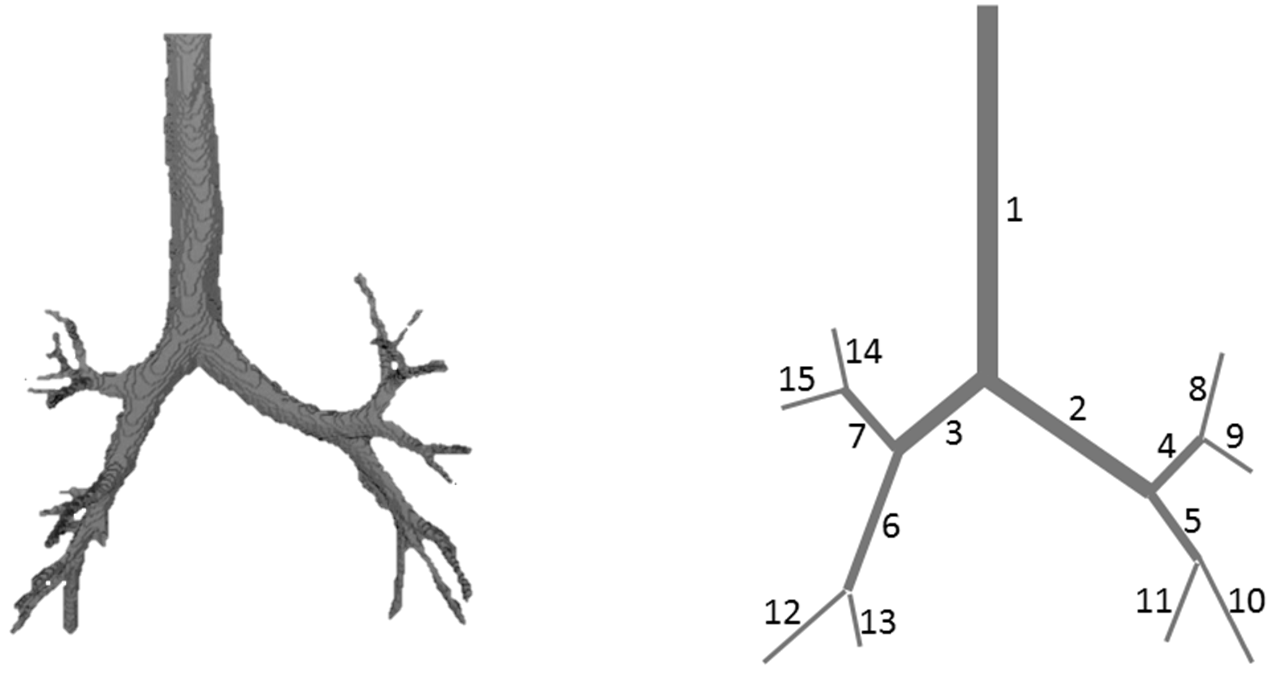
\includegraphics[scale=0.5]{ct.png}
	\caption{3D сегментация индивидуальных CT-данных трахейно-бронхиальной трубки и 1D сетевая структура на основе 3D сегментации} 
	\label{s2vechart}
\end{figure}

Поток воздуха в трахеи и бронхиальных трубках проводящей зоны легких моделируется при помощи 1D динамической модели движения несжимаемой жидкости в системе эластичных трубок в предположении о малой величине отношения диаметра к длине для каждой отдельной трубки, что позволило считать линейную скорость и давление осредненными по поперечному сечению величинами, зависящими только от координаты вдоль трубки. Поток в каждой трубке описывается с помощью уравнения сохранения масс и импульса\cite{Simakov08b,Kholodov2006}:
\begin{equation} \label{GrindEQ__1_} 
\frac{\partial S_{k} }{\partial t} +\frac{\partial \left(S_{k} u_{k} \right)}{\partial x} =0,  
\end{equation} 
\begin{equation} \label{GrindEQ__2_} 
\frac{\partial u_{k} }{\partial t} +\frac{\partial }{\partial x} \left(\frac{u_{k}^{2} }{2} +\frac{p_{k} \left(S_{k} \right)}{\rho } \right)=0,  
\end{equation} 
где $t$ ~--время; $x$ ~--координата вдоль трубки; $k$ ~--индекс бронхиальной трубки; $\rho $ ~--плотность воздуха в бронхиальных трубках (принималась за константу); $S_{k} $ ~--площадь поперечного сечения трубки; $u_{k} \left(t,x\right)$ ~--линейная скорость потока воздуха, осредненная по площади поперечного сечения $S_{k} \left(t,x\right)$; $p_{k} \left(S_{k} \right)$ ~--плотность газа в бронхиальных трубках. 

Считалось, что внутри трубок отсутствуют стоки и источники газа, а также не рассматривалось трение об стенки, гравитация и другие силы. Эластичные свойства стенок дыхательных трубок связаны с площадью поперечного сечения с помощью линейной зависимости в «уравнении состояния»: 
\begin{equation} \label{GrindEQ__3_} 
p_{k} \left(S_{k} \right)=\rho _{w} c_{0k}^{2} \left(\frac{S_{k} }{S_{0k} } -1\right),  
\end{equation} 

где $\rho _{w} $ ~-- плотность материала бронхиальных трубок; $S_{0k} $ ~-- площадь поперечного сечения бронхиальной трубки в состоянии равновесия; $c_{0k} $ ~-- скорость распространения малых возмущений в материале стенок бронхиальных трубок. 

Линейная зависимость была выбрана на основе анатомических свойств стенок бронхиальных трубок \cite{Simakov08b}.

В соответствии с анатомическими параметрами трахейно-бронхиального дерева считалось, что все бифуркации трахейных трубок имеют дихотомическую структуру: всегда состоят из одной входящей бронхиальной трубки $k_{1}^{n}  $ и двух исходящих бронхиальных трубок $k_{2,3}^{n} $. Граничные условия в точке стыковки с индексом $m$ бронхиальных трубок с индексами $k_{1}^{n} $, $k_{2}^{n} $, $k_{3}^{n} $ определяются на основе закона сохранения массы и уравнения Бернулли (разница гравитационных потенциалов незначительна):  

\begin{equation} \label{GrindEQ__4_} 
S_{k_{1}^{n} } \left(t,L_{k_{1}^{n} } \right)u_{k_{1}^{n} } \left(t,L_{k_{1}^{n} } \right)=S_{k_{2}^{n} } \left(t,0\right)u_{k_{2}^{n} } \left(t,0\right)+S_{k_{3}^{n} } \left(t,0\right)u_{k_{3}^{n} } \left(t,0\right),  
\end{equation} 
\begin{equation} \label{GrindEQ__5_} 
\frac{p_{k_{i} } \left(S_{k_{i} } \left(t,\tilde{x}_{k_{i} } \right)\right)}{\rho } +\frac{u_{k_{i} }^{2} \left(t,\tilde{x}_{k_{i} } \right)}{2} =I_{m} \left(t\right),\; i=1\div 3, 
\end{equation} 
где $\tilde{x}_{k} =L_{k} $~-- для входящих бронхиальных трубок; $\tilde{x}_{k} =0$ ~--для исходящих бронхиальных трубок, $L_{k} $ ~--длина бронхиальной трубки, $I_{n} \left(t\right)$ ~--инвариант потока.

В области входа потока газа в носоглотку используется граничное условие - постоянное давление, равное атмосферному $p_{atm} $ давлению. 
\begin{equation} \label{GrindEQ__6_} 
p_{1} \left(S_{1} \left(t,0\right)\right)=p_{atm} =const.  
\end{equation} 
В соответствии с уравнением \eqref{GrindEQ__3_}, это условие эквивалентно постоянной площади поперечного сечения трубки.

Граничные условия в области стыковки альвеолярных объемов и бронхиальных трубок основаны на уравнениях сохранения массы и равенства давлений:
\begin{equation} \label{GrindEQ__7_} 
\frac{dV_{ak} }{dt} =S_{k} \left(t,L_{k} \right)u_{k} \left(t,L_{k} \right),  
\end{equation} 
\begin{equation} \label{GrindEQ__8_} 
p_{ak} =p_{k} \left(t,L_{k} \right).  
\end{equation} 

Поскольку нижние дыхательные пути состоят из сильно разветвленной сети мелких альвеолярных объемов. Для математического описания движения воздуха использовалась модель, основанная на однокомпонентном представлении легкого, в которой суммарная масса легких и грудной клетки считается распределенной по поверхности резервуаров переменного объема, каждый из которых соединяется с одной трубкой из последнего поколения трахейно-бронхиального дерева. Механические свойства данных резервуаров определяются интегральными характеристиками:
\begin{equation} 
\label{GrindEQ__9_} 
R_{a}^{k} \frac{dV_{a}^{k} }{dt} +E_{a}^{k} \left(V_{a}^{k} -V_{0a}^{k} \right)=p_{a}^{k} -p_{pl} \left(t\right), 
\end{equation} 

\begin{equation} 
\label{GrindEQ__91_}
V_{0a}^{k} = \frac{d_{k}^{2}}{\sum_{j=8}^{15} d^{2}_{j}}V_{0}^{tot} 
\end{equation} 
где $k$ ~-- индекс альвеолярного компонента (соответствует индексу связанной терминальной бронхиальной трубкой), $V_{a}^{k} $ ~-- объем альвеолярного компонента; $V_{0a}^{k} $ ~-- объем альвеолярного компонента в не напряженном состоянии; $R_{a}^{k} $ ~-- эффективное гидравлическое сопротивление; $E_{a}^{k} $ ~--эффективная эластичность; $p_{a}^{k} $ ~--давление внутри альвеолярного компонента; $p_{pl} \left(t\right)$ ~--плевральное давление со стороны дыхательной мускулатуры, которое определяется из параметров дыхания; $V_{0}^{tot} $ ~-- суммарный объем легких в не напряженном состоянии. 

В случая нормального дыхания плевральное давление определяется синусоидальной зависимостью:
\begin{equation} \label{GrindEQ__10_} 
p_{pl} \left(t\right)=p_{g} \sin \left(\nu t\right), 
\end{equation} 
где $\nu $ ~--чистота дыхания; $p_{g} $ ~-- амплитуда плеврального давления со стороны дыхательной мускулатуры. Предполагалось, что материал альвеолярных компонент линейно-упругий, таким образом $E_{a}^{k} $ ~--постоянная. Эффективное гидравлическое сопротивление $R_{a}^{k} $ оценивалось на основе закона Пуазейля для трубки:
\begin{equation} \label{GrindEQ__11_} 
R_{a} =\frac{8\eta l_{ef} }{\pi r_{ef}^{4} } ,  
\end{equation} 
где  эффективные длинна $l_{ef} $ и радиус $r_{ef} $ могут быть оценены на основе равенства объемов у соответствующих сферы и цилиндра:
\begin{equation} \label{GrindEQ__12_} 
V_{a} \approx \pi r_{ef}^{2} l_{ef} \approx \frac{4\pi r_{ef}^{3} }{3} .  
\end{equation} 
В итоге, уравнение \eqref{GrindEQ__12_} упрощается до выражения:
\begin{equation} \label{GrindEQ__13_} 
R_{a} =\frac{128\eta }{9\pi ^{2} V_{a} }  
\end{equation} 
и подставляется в уравнение \eqref{GrindEQ__9_}.

Граничные условия в точках бифуркаций бронхиальных трубок уравнения \eqref{GrindEQ__4_}, \eqref{GrindEQ__5_}, в области входа потока газа в носоглотку уравнения \eqref{GrindEQ__6_}, а также в точках соединения с соответствующими альвеолярными компонентами уравнения \eqref{GrindEQ__7_}-\eqref{GrindEQ__10_} могут быть дополнены условиями совместности вдоль характеристик системы гиперболических уравнений \eqref{GrindEQ__1_}, \eqref{GrindEQ__2_}, выходящих из области интегрирования \cite{Simakov08b,Kholodov2006}. Используя обозначения 
\begin{equation} \label{GrindEQ__14_} 
V_{k} =\left(\begin{array}{c} {S_{k} } \\ {u_{k} } \end{array}\right),\; F\left(V_{k} \right)=\left(\begin{array}{c} {S_{k} u_{k} } \\ {\frac{u_{k}^{2} }{2} +\frac{p_{k} \left(S_{k} \right)}{\rho } } \end{array}\right),  
\end{equation} 
можно переписать уравнения \eqref{GrindEQ__1_},\eqref{GrindEQ__2_} в дивергентной форме:
\begin{equation} \label{GrindEQ__15_} 
\frac{\partial V_{k} }{\partial t} +\frac{\partial F\left(V_{k} \right)}{\partial x} =0 
\end{equation} 
Собственные значения $\lambda _{k} $ и левые собственные вектора $w_{k} $ матрицы Якоби $A_{k} =\frac{\partial F_{k} }{\partial V_{k} } =\left\{\frac{\partial F_{ki} }{\partial V_{kj} } \right\}_{i,j=1}^{2} $:
\begin{equation} \label{GrindEQ__16_} 
\lambda _{ki} =u_{k} +\left(-1\right)^{i} \sqrt{\frac{S_{k} }{\rho } \frac{\partial p_{k} }{\partial S_{k} } } =u_{k} +\left(-1\right)^{i} c_{0k} \sqrt{\frac{S_{k} }{S_{0k} } } ,\; i=1,2,  
\end{equation} 
\begin{equation} \label{GrindEQ__17_} 
w_{ki} =\left(\begin{array}{c} {\sqrt{\frac{1}{\rho } \frac{\partial p_{k} }{\partial S_{k} } } } \\ {\left(-1\right)^{i} \sqrt{S_{k} } } \end{array}\right)=\left(\begin{array}{c} {\frac{c_{0k} }{\sqrt{S_{0k} } } } \\ {\left(-1\right)^{i} \sqrt{S_{k} } } \end{array}\right), i=1,2.  
\end{equation} 
Уравнения условий совместности \eqref{GrindEQ__1_},\eqref{GrindEQ__2_} вдоль характеристик:
\begin{equation} \label{GrindEQ__18_} 
w_{ki} \cdot \left(\frac{dV_{k} }{dt} \right)_{i} =w_{ki} \cdot \left(\frac{\partial V_{k} }{\partial t} +\lambda _{ki} \frac{\partial V_{k} }{\partial x} \right)=0, i=1,2 
\end{equation} 

В случае дыхательной механики как для нормальных, так и патологических условий выполнено неравенство $\left|u_{k} \right|<c_{0k} \sqrt{\frac{S_{k} }{S_{0k} } } $, а также существует одно отрицательное и одно положительное собственное значение, одна входящая и одна выходящая характеристика на входе и выходе каждой бронхиальной трубки. Каждый набор граничных условий, описанный выше, должен быть связан с уравнением \eqref{GrindEQ__18_} для каждой входящей и выходящей трубки. Для входящей трубки должно использоваться положительное собственное значение ($i=2$, положительный наклон), для исходящей трубки должно использоваться отрицательное собственное значение ($i=1$, отрицательный наклон).

\subsection{Модель переноса кислорода и углекислого газа в легких}

Транспорт кислорода и углекислого газа в легких описывается 1D уравнением конвективно-диффузионного переноса:
\begin{equation} \label{GrindEQ__19_} 
\frac{\partial C_{k,m} }{\partial t} +u_{k} \frac{\partial C_{k,m} }{\partial x} =0  
\end{equation} 
где $m$ ~-- индекс вещества; $C_{k,m} $ ~-- доля(концентрация) вещества $m$ в $k^{ой} $ бронхиальной трубке, $D_{m} $ ~-- коэффициент диффузии вещества $m$. 

Граничные условия в точках бифуркаций бронхиальных трубок определяются из условий сохранения массы:
\begin{equation} \label{GrindEQ__20_} 
\begin{array}{l} {C_{k_{1}^{p} ,m} \left(t,L_{k_{1}^{p} } \right)S_{k_{1}^{p} } \left(t,L_{k_{1}^{p} } \right)u_{k_{1}^{p} } \left(t,L_{k_{1}^{p} } \right)=} \\ {\; \; \; \; \; \; \; \; \; \; \; \; \; \; \; \; \; \; \; \; \; \; \; \; =C_{k_{2}^{p} ,m} \left(t,0\right)S_{k_{2}^{p} } \left(t,0\right)u_{k_{2}^{p} } \left(t,0\right)+C_{k_{3}^{p} ,m} \left(t,0\right)S_{k_{3}^{p} } \left(t,0\right)u_{k_{3}^{p} } \left(t,0\right)} \end{array}.  
\end{equation} 
При этом использовалось предположение о пространственной малости области стыковок и как следствие малости вклада диффузионного члена.

Если $u_{k_{j}^{p} } \left(t,\tilde{x}_{k_{j}^{p} } \right)>0$, то $C_{k_{j}^{p} ,m} $ определяется из уравнения \eqref{GrindEQ__19_} вдоль выходящей характеристики. Если $u_{k_{j}^{p} } \left(t,\tilde{x}_{k_{j}^{p} } \right)<0$, то 
\begin{equation}  
C_{k_{j}^{p} ,m} \left(t,\tilde{x}_{k_{j}^{p} } \right)=C_{p,m}^{node} ,  
\end{equation} 
где $C_{p,m}^{node} $ ~-- концентрация в $p^{ой} $ точке бифуркации бронхиальных трубок, которая определяется из уравнения \eqref{GrindEQ__20_}. Граничные условия на входе в носоглотку во время вдоха $\left(u_{1} \left(t,0\right)>0\right)$ определяются из условий: 
\begin{equation} \label{GrindEQ__22_} 
C_{1,O_{2} } \left(t,0\right)=C_{O_{2} }^{atm} , C_{1,CO_{2} } \left(t,0\right)=C_{CO_{2} }^{atm} ,  
\end{equation} 
или из уравнения \eqref{GrindEQ__19_} в случае $u_{1} \left(t,0\right)<0$ (выдох).

На выходе из терминальных бронхиальных трубок концентрация $C_{k,m} \left(t,L_{k} \right)$ определяется из выражения \eqref{GrindEQ__19_}, если $u_{k} \left(t,L_{k} \right)>0$ или вычисляется совместно с моделью газообмена между альвеолярным компонентом и кровеносной системой:

 $C_{k,m} \left(t,L_{k} \right)=C_{a,m}^{k} $, если $u_{k} \left(t,L_{k} \right)<0$
\begin{equation} \label{GrindEQ__24_} 
\frac{d\left(C_{a,m}^{k} V_{a}^{k} \right)}{dt} =C_{k,m} S_{k} \left(t,L_{k} \right)u_{k} \left(t,L_{k} \right)+D_{m} S_{a}^{k} \left(C_{m}^{b} -C_{a,m}^{k} \right),  
\end{equation} 
\begin{equation} \label{GrindEQ__25_} 
\frac{dC_{m}^{b} }{dt} =\frac{Q_{m}^{b} }{V^{b} } +D_{m} \sum _{k}\frac{S_{a}^{k} }{V^{b} } \left(C_{a,m}^{k} -C_{m}^{b} \right) ,  
\end{equation} 
где $k$ ~-- набор индексов альвеолярных компонент (в данной работе $k=8,...,15$); $C_{a,m}^{k} $ ~-- концентрация $m^{го} $  вещества в $k^{м} $ альвеолярном компоненте; $D_{m} $ ~-- коэффициент диффузии $m^{го} $ вещества между альвеолярным компонентом и кровеносной системой; $C_{m}^{b} $  ~-- концентрация $m^{го} $ вещества в кровеносной системе; $Q_{m}^{b} $ ~-- сток или источник $m^{го} $ вещества, соответствующий физиологическим данным в организме; $V^{b} $ ~-- полный объем крови в организме человека; $S_{a}^{k} $ ~-- эффективная площадь поверхности альвеолярного компонента, которая определяется из выражения:
\begin{equation} \label{GrindEQ__26_} 
S_{a}^{k} =\sqrt[{3}]{36\pi \left(V_{a}^{k} \right)^{2} } .  
\end{equation} 

\subsection{Усредненная модель легких}
\label{sec:lumpLung}
Для ряда практических задач не требуется очень детальное описание воздушных потоков в легких, а необходимо воспроизводить только общую интегральную динамику. Для данных задач использовалась усредненная модель, для которой можно получить аналитическое решение. Для реализации модели необходимо минимальное количество вычислительных ресурсов. Уравнение динамики объема легких в линейном приближении:
\begin{equation}\label{AlvEq}
R\frac{dV}{dt}+E(V-V_{0})=P_{g}\sin wt,
\end{equation}
\noindent где \( R\)~--- сопротивление дыхательных путей, \( E\) --- эластичность легких, \( V_{0}\) ~--- объем резервуара в не напряженном состоянии, \( w\) ~--- частота дыхания, \( P_{g}\)~---плевральное давление, \( t\) ~--- время. 

Дифференциальное уравнение (\ref{AlvEq}) имеет аналитическое решение, состоящее из постоянной, синусоидальной и экспоненциально затухающей компонент:
\begin{equation}\label{V_analyt}
V\left(t\right)=V_{0}+\frac{P_{g}}{R\sqrt{\lambda^2+w^2}}\sin \left( wt-\arctg\frac{w}{\lambda} \right)+\frac{P_{g}w}{R\left(\lambda^2+w^2\right)}e^{-\lambda t}, \lambda=\frac{E}{R}.
\end{equation}
Из (\ref{V_analyt}) в частности следует, что в установившемся квазипериодическом режиме дыхательный объем \( V_{T}\) определяется выражением:
\begin{equation}
V_{T}=\frac{2P_{g}}{R\sqrt{\lambda^2+w^2}}.
\end{equation}

Далее предполагается, что газообмен между кровеносной системой и легкими происходит за счет диффузии и пропорционален разности парциальных давлений дыхательных газов. Концентрация \(O_{2}\) и \( CO_{2}\) в легочном отделе кровеносной системы определяется из уравнения:
\begin{equation}\label{lungMatter1}
\frac{d\left(C_{i}V\right)}{dt}  = Q_{i}+D_{i}S\left(P_{i}-P_{i,b}\right),
\end{equation}
\begin{equation}\label{lungMatter2}
Q_{i}= \begin{cases} \displaystyle
C_{i}^{air}\frac{dV}{dt}, \frac{dV}{dt} \ge 0 \\
\displaystyle
C_{i}\frac{dV}{dt},  \frac{dV}{dt} <0
\end{cases},
\end{equation}
\begin{equation}
S =\sqrt[{3}]{36\pi \left(V \right)^{2} }
\end{equation}
\noindent где \(C_{i}\)~--- концентрация $i$-го вещества в легких, 
\( C_{i}^{air}\)~--- концентрация $i$-го вещества в атмосфере, 
\( D_{i}\)~--- коэффициент диффузии между легкими и кровью для $i$-ого вещества, 
\( P_{i}\)~--- парциальное давление $i$-го вещества в легких, 
\( P_{i,b}\)~--- парциальное давление $i$-го вещества в крови, \( S\)~--- площадь поверхности контакта между легкими и кровеносной системой. 

\subsection{Модель регуляции дыхания}
\label{sec:lung_reg}
Значительные и/или длительные отклонения от нормальных значений концентраций $O_{2}$ и $CO_{2}$ в артериальной и венозной крови могут приводить к существенным патологическим изменениям, таким, как недостаток кислорода (гипоксия и ишемические явления), изменение кислотно-щелочного баланса крови (ацидоз или алкалоз) и др. При значительных и/или длительных отклонения эти и другие процессы могут стать необратимыми.
В условиях меняющейся внешней среды и внутреннего состояния организма действие его регуляторных систем направлено на поддержание гомеостаза --- сохранение нормальных значений различных показателей. Основным фактором, определяющим активность респираторной функции, считается отклонение парциальных давлений $O_{2}$ и $CO_{2}$ в крови, вызывающих активацию соответствующих рецепторов нервной системы. При этом отдельно выделяется функция рецепторов спинномозгового отдела(центральные хеморецепторы) и синуса сонной артерии(периферические хеморецепторы).
Среди других механизмов управления респираторной активностью выделяют прогностическую подстройку на основе текущего состояния (например, уровня физической нагрузки) \cite{volkov2013}.

Действие центральных и периферических хеморецепторы различны.
Центральные хеморецепторы активируются при отклонении парциального давления $CO_{2}$ в спинномозговой жидкости и церебральном отделе кровообращения. Периферические хеморецепторы активируются при отклонении парциальных давлений $O_{2}$ и $CO_{2}$ в области дуги аорты и синуса сонной артерии \cite{wolf2007}.

Вклады центральных и периферических хеморецепторов считаются независимыми друг от друга. Регуляция минутной вентиляции: 
\begin{equation}\label{VentReg}
V_{E}=V_{SS}+\left(V_{C}+V_{P}\right)\left(1-e^{-\frac{t}{\tau}}\right),
\end{equation}
где \( V_{E}\)~--- минутная вентиляция легких, 
\( V_{SS}\)~--- минутная вентиляция легких в норме, 
\( V_{C}\)~--- регуляторный вклад центральных хеморецепторов,
\( V_{P}\)~--- регуляторный вклад периферических хеморецепторов,
\( \tau\)~--- параметр времени установления нового значения вентиляции. 
Активность центральных хеморецепторов определяется отклонением парциального давления  $CO_{2}$ от условно нормального значения~\cite{wolf2007}:
\begin{equation}
V_{C}=K_{cCO_{2}}\left(P_{cCO_{2}}-T_{cCO_{2}} \right), V_{C}\ge 0,
\end{equation}
\noindent где \( P_{cCO_{2}}\)~--- парциальное давление $CO_{2}$ в отделе центральных хеморецепторов, 
\( T_{cCO_{2}}\)~--- условно нормальное значение парциального давления $CO_{2}$ в отделе центральных хеморецепторов, 
\( K_{cCO_{2}}\)~--- коэффициент пропорциональности.

Регуляция минутной вентиляции периферическими хеморецепторами линейно зависит от парциального давления \( CO_{2}\), и обратно пропорциональна гипоксическому воздействию (снижению парциального давления \( O_{2}\) ). Однако, дыхательная реакция на острую гипоксию имеет двухфазный характер: с одной стороны, снижение величины парциального давления \( O_{2}\) приводит к повышению вентиляции, с другой стороны это приводит к  повышенному вымыванию \( CO_{2}\) и, как следствие, к снижению гиперкапнического стимула с соответствующим снижением вентиляции. Данный эффект эмпирически описан в~\cite{wolf2007} в виде:   
\begin{equation}
V_{P}=K_{pCO_{2}}\left(P_{pCO_{2}}-T_{pCO_{2}} \right)+\left(\frac{570}{P_{pO_{2}}-26.2}-8.05\right)F(P_{pCO_{2}}), V_{P}\ge 0,
\end{equation}
\begin{equation}
F(P_{pCO_{2}})=\begin{cases}
\left(5-4N_{pCO_{2}}^4 \right)^{-1}, & N_{pCO_{2}}\le 1 \\
N_{pCO_{2}}^3, & N_{pCO_{2}}> 1 
\end{cases}, 
N_{pCO_{2}}=\frac{P_{pCO_{2}}}{P_{pCO_{2}}^0},
\end{equation}
\noindent где \( T_{pCO_{2}}\) ~--- условно нормальное значение парциального давления $CO_{2}$ в отделе периферических хеморецепторов, 
\( K_{pCO_{2}}\)~--- коэффициент пропорциональности, 
\( P_{pO_{2}}, P_{pCO_{2}}\)~--- значения парциальных давлений $O_{2}$ и $CO_{2}$ в отделе периферических хеморецепторов,
\( P_{pCO_{2}}^0\)~--- референтное значение парциального давления $CO_{2}$ в отделе периферических хеморецепторов в норме. 

Минутная вентиляция легких зависит от дыхательного объема и количества дыхательных циклов в минуту:
\begin{equation}
V_{E}=nV_{T},
\end{equation}
\noindent где \( n\)  ~---  количество дыхательных циклов в минуту, \( V_{T}\)~--- дыхательный объем. Таким образом, одинаковые значения минутной вентиляции легких могут быть получены при различных значениях дыхательного объема и количестве дыхательных циклов в минуту.

Лабораторные исследования показали, что незначительное увеличение минутной вентиляции $\left( V_E \le V_{E,T} \right)$ обеспечивается организмом за счет увеличения дыхательного объема. Частота дыхания при этом остается постоянной. При заметных отклонениях состава крови, приводящих к условию $V_E > V_{E,T}$, компенсаторные возможности за счет дыхательного объема достигают предела и минутная вентиляции увеличивается как за счет изменения дыхательного объема, так и за счет частоты дыхания \cite{volkov2013}:
\begin{equation} \label{nVt}
\begin{cases}
n=n_{0},\; V_{T}=\frac{\displaystyle V_{E}}{\displaystyle n_{0}}; & V_{E} \le V_{E,T}  \\
V_{T}=\alpha V_{E}^{\displaystyle \beta},\; n= \frac{\displaystyle V_{E}}{\displaystyle V_{T}}; & V_{E} > V_{E,T}
\end{cases},
\end{equation}
\noindent где \( n_{0}\) ~---  частота дыхательных циклов в минуту в норме, 
\( V_{E,T}\)~--- пороговое значение минутной вентиляции, 
\( \alpha\) и \( \beta\)~--- постоянные коэффициенты.

Значение констант модели регуляции дыхательного объема приведены в таблице~\ref{tab:params_reg}.

\subsection{Общая структура OD-1D модели}

Поток воздуха в верхних дыхательных путях описываются уравнениями сохранения массы и импульса в каждой отдельной трубке \eqref{GrindEQ__1_},\eqref{GrindEQ__2_}:
\begin{equation} 
\frac{\partial S_{k} }{\partial t} +\frac{\partial \left(S_{k} u_{k} \right)}{\partial x} =0 \notag
\end{equation} 
\begin{equation} 
\frac{\partial u_{k} }{\partial t} +\frac{\partial }{\partial x} \left(\frac{u_{k}^{2} }{2} +\frac{p_{k} \left(S_{k} \right)}{\rho } \right)=0 \notag  
\end{equation} 

Система дополняется "уравнением состояния" \eqref{GrindEQ__3_}:
\begin{equation} 
p_{k} \left(S_{k} \right)=\rho _{w} c_{0k}^{2} \left(\frac{S_{k} }{S_{0k} } -1\right)\notag  
\end{equation} 
Граничное условие в области входа потока газа в носоглотку \eqref{GrindEQ__6_}: 
\begin{equation}
p_{1} \left(S_{1} \left(t,0\right)\right)=p_{atm} =const. \notag 
\end{equation} 
Граничные условия в точке стыковки бронхиальных трубок определяются из закона сохранения массы и уравнения Бернулли \eqref{GrindEQ__4_}, \eqref{GrindEQ__5_}:  

\begin{equation} 
S_{k_{1}^{n} } \left(t,L_{k_{1}^{n} } \right)u_{k_{1}^{n} } \left(t,L_{k_{1}^{n} } \right)=S_{k_{2}^{n} } \left(t,0\right)u_{k_{2}^{n} } \left(t,0\right)+S_{k_{3}^{n} } \left(t,0\right)u_{k_{3}^{n} } \left(t,0\right)\notag
\end{equation} 
\begin{equation} 
\frac{p_{k_{i} } \left(S_{k_{i} } \left(t,\tilde{x}_{k_{i} } \right)\right)}{\rho } +\frac{u_{k_{i} }^{2} \left(t,\tilde{x}_{k_{i} } \right)}{2} =I_{m} \left(t\right),\; i=1\div 3\notag 
\end{equation} 

Движение воздуха в переходной зоне описывается интегральной моделью для каждого альвеолярного объема \eqref{GrindEQ__9_}, \eqref{GrindEQ__91_}:
\begin{equation} 
\frac{128\eta }{9\pi ^{2} V_{a}^{k} } \frac{dV_{a}^{k} }{dt} +E_{a}^{k} \left(V_{a}^{k} -V_{0a}^{k} \right)=p_{a}^{k} -p_{pl} \left(t\right) \notag
\end{equation} 
\begin{equation} 
V_{0a}^{k} = \frac{d_{k}^{2}}{\sum_{j=8}^{15} d^{2}_{j}}V_{0}^{tot} \notag
\end{equation}

Граничные условия в области стыковки альвеолярных объемов и бронхиальных трубок определяются из уравнений сохранения массы и равенства давлений \eqref{GrindEQ__7_}, \eqref{GrindEQ__8_}:
\begin{equation} 
\frac{dV_{ak} }{dt} =S_{k} \left(t,L_{k} \right)u_{k} \left(t,L_{k} \right)\notag  
\end{equation} 
\begin{equation} 
p_{ak} =p_{k} \left(t,L_{k} \right)\notag 
\end{equation} 

Перенос $O_{2}$ и $CO_{2}$ в верхних дыхательных путях описывается конвективным уравнением \eqref{GrindEQ__19_}: 
\begin{equation}
\frac{\partial C_{k,m} }{\partial t} +u_{k} \frac{\partial C_{k,m} }{\partial x} =0\notag 
\end{equation} 

Граничные условия для концентраций  в области входа потока газа в носоглотку во время вдоха $\left(u_{1} \left(t,0\right)>0\right)$: 
\begin{equation} 
C_{1,O_{2} } \left(t,0\right)=C_{O_{2} }^{atm} , C_{1,CO_{2} } \left(t,0\right)=C_{CO_{2} }^{atm} \notag
\end{equation} 
в случае $u_{1} \left(t,0\right)<0$ (выдох) значения концентраций определяются из уравнения \eqref{GrindEQ__19_} .

Граничные условия в точках бифуркаций бронхиальных трубок определяются из закона сохранения массы \eqref{GrindEQ__20_}:
\begin{equation} 
\begin{array}{l} {C_{k_{1}^{p} ,m} \left(t,L_{k_{1}^{p} } \right)S_{k_{1}^{p} } \left(t,L_{k_{1}^{p} } \right)u_{k_{1}^{p} } \left(t,L_{k_{1}^{p} } \right)=} \\ {\; \; \; \; \; \; \; \; \; \; \; \; \; \; \; \; \; \; \; \; \; \; \; \; =C_{k_{2}^{p} ,m} \left(t,0\right)S_{k_{2}^{p} } \left(t,0\right)u_{k_{2}^{p} } \left(t,0\right)+C_{k_{3}^{p} ,m} \left(t,0\right)S_{k_{3}^{p} } \left(t,0\right)u_{k_{3}^{p} } \left(t,0\right)} \end{array}.  \notag 
\end{equation} 

Если $u_{k_{j}^{p} } \left(t,\tilde{x}_{k_{j}^{p} } \right)>0$, то $C_{k_{j}^{p} ,m} $ определяется из уравнения \eqref{GrindEQ__19_} вдоль выходящей характеристики. Если $u_{k_{j}^{p} } \left(t,\tilde{x}_{k_{j}^{p} } \right)<0$, то $ C_{k_{j}^{p} ,m} \left(t,\tilde{x}_{k_{j}^{p} } \right)=C_{p,m}^{node}$ 



Уравнение концентраций в альвеолярных объемах \eqref{GrindEQ__24_}:
\begin{equation}  
\frac{d\left(C_{a,m}^{k} V_{a}^{k} \right)}{dt} =C_{k,m} S_{k} \left(t,L_{k} \right)u_{k} \left(t,L_{k} \right)+D_{m} S_{a}^{k} \left(C_{m}^{b} -C_{a,m}^{k} \right)\notag  
\end{equation} 
Уравнение концентрации в кровеносной системе(однокомпонентная модель) \eqref{GrindEQ__25_}:
\begin{equation} 
\frac{dC_{m}^{b} }{dt} =\frac{Q_{m}^{b} }{V^{b} } +D_{m} \sum _{k}\frac{S_{a}^{k} }{V^{b} } \left(C_{a,m}^{k} -C_{m}^{b} \right)\notag  
\end{equation}
\textit{Примечание: модель регуляции (Раздел \ref{sec:lung_reg}) не применялась для совместных расчетов с 0D-1D моделью (модель регуляции использовалась совместно с усредненной моделью (Раздел \ref{sec:lumpLung}), моделями кровеносной системы и мышечного метаболизма (Глава \ref{chapt:blood_muscle})})

\subsection{Допущения модели}
Предполагается, что дыхательный поток в дыхательных путях имеет, в основном, ламинарный характер. Состав дыхательного газа в альвеолярном объеме однородный, а сам газ несжимаем. Также предполагается, что при поступлении в легкие из внешней среды газ мгновенно нагревается и далее его температура постоянна, при этом происходит его мгновенное насыщение водяными парами.   

\section{Численные методы}
\subsection{Численная реализация модели движения воздуха}

Движение дыхательных газов для каждой бронхиальной трубки описывается с помощью системы нелинейных гиперболических уравнений \eqref{GrindEQ__1_},\eqref{GrindEQ__2_}. Данные пары уравнений для трубок объединены нелинейными алгебраическими уравнениями, которые получены из граничных условий на входе \eqref{GrindEQ__6_} в носоглотку или конечно-разностной аппроксимации граничных условий на выходе \eqref{GrindEQ__7_}-\eqref{GrindEQ__9_} из альвеолярных объемов, в точках бифуркаций бронхиальных трубок \eqref{GrindEQ__4_},\eqref{GrindEQ__5_}. Каждая система дополнена конечно-разностной аппроксимацией соответствующих условий совместности \eqref{GrindEQ__18_} в каждом вышеуказанном случае. 

Численный алгоритм позволяет разделить расчет на каждом шаге по времени на несколько этапов.  На первом этапе решаются уравнения \eqref{GrindEQ__1_},\eqref{GrindEQ__2_} во внутренних узлах расчетной сетки для каждой бронхиальной трубки. Используется сеточно-характеристический метод \cite{Magomedov1988} для расчета динамики газов в верхних дыхательных путях \cite{kholodov2001,Vassilevski2011,Bessonov2016}. На втором этапе с помощью метода Ньютона решается система нелинейных алгебраических уравнений на входах, выходах, точках бифуркаций для каждой бронхиальной трубки в граничных узлах расчетной сетки. Данная система получается из конечно-разностной  аппроксимации уравнений \eqref{GrindEQ__18_}, в которых используются значения в соседних с граничными узлами расчетной сетки, полученные на первом этапе численного алгоритма. Начальное приближение для итерационной процедуры берется с предыдущего шага по времени. На практике понадобилось не более 5 итераций для достижения сходимости на каждом шаге по времени с использованием относительной точности $10^{-6} $ для всех численных экспериментов в данной работе. Обзор других возможных подходов к данной задаче описан в \cite{kholodov2001}. Основная разница численной реализации алгоритма для данной работы связаны с аппроксимацией системы граничных условий \eqref{GrindEQ__4_} -- \eqref{GrindEQ__9_}; условий совместности \eqref{GrindEQ__18_} и модели переноса дыхательных газов \eqref{GrindEQ__19_} -- \eqref{GrindEQ__26_}. 

При численном решении данной системы с одной стороны должна быть учтена возможность возникновения ударных волн в системе, а с другой стороны используемый численный метод должен быть достаточно экономичным. В данной работе использовалась явная двухшаговая гибридная схема, соответствующая наиболее точной монотонной схеме первого порядка и наименее осциллирующей схеме второго порядка точности \cite{Magomedov1988}:

\begin{equation}
\tilde{V}_{m} =V_{m}^{n} -\tau \left(F_{m+1}^{n} -F_{m-1}^{n} \right)/2h
\end{equation} 
\begin{equation}
\begin{array}{l} 
{V_{m}^{n+1} =\tilde{V}_{m} +\left[\left(\mathbf{\Omega} ^{-1} \mathbf{B}\mathbf{\Omega} \right)_{m+1/2} \left(V_{m+1}^{n} -V_{m}^{n} \right)-\left(\mathbf{\Omega} ^{-1} \mathbf{B}\mathbf{\Omega} \right)_{m-1/2} \left(V_{m}^{n} -V_{m-1}^{n} \right)\right]+} \\ {+\left[\left(\mathbf{\Omega} ^{-1} \mathbf{C}\mathbf{\Omega} \right)_{m+1/2} \left(\tilde{V}_{m+1} -\tilde{V}_{m} \right)-\left(\mathbf{\Omega} ^{-1} \mathbf{C}\mathbf{\Omega} \right)_{m-1/2} \left(\tilde{V}_{m} -\tilde{V}_{m-1} \right)\right]+} \\ {+\left(\mathbf{\Omega} ^{-1} \mathbf{D}\mathbf{\Omega} \right)_{m+1/2} \left(\tilde{V}_{m+1} +\tilde{V}_{m} -V_{m+1}^{n} -V_{m}^{n} \right)-} \\ {-\left(\mathbf{\Omega} ^{-1} \mathbf{D}\mathbf{\Omega} \right)_{m-1/2} \left(\tilde{V}_{m} +\tilde{V}_{m-1} -V_{m}^{n} -V_{m-1}^{n} \right)} 
\end{array}
\end{equation}
где $\tau $ ~-- шаг по времени; $h $ ~-- равномерный шаг по пространству; $\mathbf{\Omega}$ ~-- матрица, состоящая из левых собственных векторов якобиана системы.

$ \mathbf{B}$, $\mathbf{C}$, $\mathbf{D}$ -диагональные матрицы, элементы которых при $\left|\sigma _{i} \right|\le 1,(i=1,2)$ имеют вид:
\begin{equation}
\begin{array}{l} \displaystyle {b_{i} =\frac{1}{\left|\sigma _{i} \right|} -\frac{1}{2} \left[\left|\sigma _{i} \right|+5\frac{\left(1-\gamma \right)\left(1-\left|\sigma _{i} \right|\right)\left(2-\left|\sigma _{i} \right|\right)}{19} \right]} \\ \displaystyle {c_{i} =\frac{\left(\left|\sigma _{i} \right|-1\right)}{\left|\sigma _{i} \right|} } \\ \displaystyle {d_{i} =\left[1-\frac{6\left(1-\gamma \right)\left(2-\left|\sigma _{i} \right|\right)}{19} \right]\frac{\left(1-\left|\sigma _{i} \right|\right)}{\sigma _{i} } } \end{array}
\end{equation}

При $\displaystyle \sigma _{i} =\frac{\lambda _{i} \tau }{h} $:
\begin{equation}
\begin{array}{l} \displaystyle {b_{i} =\frac{1}{\left|\sigma _{i} \right|} -\frac{1}{2} \left[\left|\sigma _{i} \right|+5\frac{\left(1-\gamma \right)\left(1-\left|\sigma _{i} \right|\right)\left(2-\left|\sigma _{i} \right|\right)}{19} \right]} \\ \displaystyle{ c_{i} = \frac{\left(\left|\sigma _{i} \right|-1\right)}{\left|\sigma _{i} \right|} } \\ \displaystyle{d_{i} =\left[1-\frac{6\left(1-\gamma \right)\left(2-\left|\sigma _{i} \right|\right)}{19} \right]\frac{\left(1-\left|\sigma _{i} \right|\right)}{\sigma _{i} } } \end{array}
\end{equation}
где $\displaystyle \tau_{i} = \frac{\lambda_{i} \tau}{h}$

При $\gamma =1$ схема является монотонной, а при $\gamma =0$ имеет второй порядок точности.

Выполняется дискретизация условий совместности \eqref{GrindEQ__18_} с помощью неявной аппроксимации первого порядка точности с использованием прямой разности для входа в бронхиальную трубку $\left(x_{k} =0\right)$ и обратной разности для выхода из бронхиальной трубки $\left(x_{k} =L_{k} \right)$ вдоль оси $x$:
\begin{equation} \label{GrindEQ__27_} 
\left(\frac{\partial V}{\partial x} \right)_{0}^{n+1} =\frac{V_{1}^{n+1} -V_{0}^{n+1} }{h} , \left(\frac{\partial V}{\partial x} \right)_{J}^{n+1} =\frac{V_{J}^{n+1} -V_{J-1}^{n+1} }{h} ,  
\end{equation} 
\begin{equation} \label{GrindEQ__28_} 
\left(\frac{\partial V}{\partial t} \right)_{p}^{n+1} =\frac{V_{p}^{n+1} -V_{p}^{n} }{\tau _{n+1} } ,\; p=0,J,  
\end{equation} 
где $V_{p}^{n} $ ~-- элемент сеточной функции, которая является аналогом для функции  $V$ из уравнения \eqref{GrindEQ__14_}. Используется равномерная расчетная сетка вдоль оси $x$:
\begin{equation} \label{GrindEQ__29_} 
\left(x_{j} ,t_{n} \right):x_{j} =hj;j=0,...,J;hJ=L;t_{n} =\sum _{p=0}^{n-1}\tau _{p}  .  
\end{equation} 
Шаг по времени выбирается на основе условий устойчивости численного метода, полученного для уравнений \eqref{GrindEQ__1_},\eqref{GrindEQ__2_}:
\begin{equation} \label{GrindEQ__30_} 
\tau _{n+1} =0.9\mathop{\max }\limits_{k=1,...,K;i=1,2} \frac{\left|\lambda _{ki}^{n} \right|}{h_{k} } ,  
\end{equation} 
где $K$ ~-- полное число бронхиальных трубок. 

Таким образом, для уравнения \eqref{GrindEQ__18_} может быть выполнена дискретизация:
\begin{equation} \label{GrindEQ__31_} 
\left(w_{i} \right)_{p}^{n} \cdot \left(\frac{V_{p}^{n+1} -V_{p}^{n} }{\tau _{n+1} } +\left(\lambda _{i} \right)_{p}^{n} \frac{V_{p}^{n+1} -V_{q}^{n+1} }{h} \right)=0,\; \left(i,p,q\right)\in \left\{\left(1,0,1\right),\left(2,J,J-1\right)\right\}.  
\end{equation} 
Также существует очевидное взаимно-однозначное соответствие между $p$ и набором трех чисел $\left(i,p,q\right)$. Таким образом, используется короткое обозначение $p=0,J$ вместо полного обозначения $\left(i,p,q\right)$. С использованием данного обозначения:
\begin{equation} \label{GrindEQ__32_} 
\alpha _{p}^{n+1} =\frac{\left(-1\right)^{i+1} c_{0} }{\sqrt{S_{p}^{n} S_{0} } } 
\end{equation} 
\begin{equation} 
\beta _{p}^{n+1} =\frac{u_{p}^{n} +\left(-1\right)^{i} \sigma _{p}^{n} u_{q}^{n+1} -\alpha _{p}^{n+1} \left(S_{p}^{n} +\left(-1\right)^{i} \sigma _{p}^{n} S_{q}^{n+1} \right)}{1+\left(-1\right)^{i} \sigma _{p}^{n} } , \sigma _{p}^{n} =\frac{\tau _{n+1} }{h} \left(\lambda _{i} \right)_{p}^{n}  \notag
\end{equation} 
Уравнение \eqref{GrindEQ__31_} может быть переписано в виде:
\begin{equation} \label{GrindEQ__33_} 
u_{p}^{n+1} =\alpha _{p}^{n+1} S_{p}^{n+1} +\beta _{p}^{n+1} ,\; p=0,J.  
\end{equation} 

Порядок аппроксимации по пространству может быть повышен до второго:
\begin{equation} \label{GrindEQ__31_2order} 
\left(w_{i} \right)_{p}^{n} \cdot \left(\frac{V_{p}^{n+1} -V_{p}^{n} }{\tau _{n+1} } +(-1)^{i}\left(\lambda _{i} \right)_{p}^{n} \frac{3V_{p}^{n+1}-4V_{q}^{n+1}+V_{z}^{n+1}}{2h} \right)=0 
\end{equation} 
\begin{equation}
\left(i,p,q,z\right)\in \left\{\left(1,0,1,2\right),\left(2,J,J-1,J-2\right)\right\} \notag
\end{equation}

\begin{equation}
 \alpha _{p}^{n+1} =\frac{\left(-1\right)^{i+1} c_{0} }{\sqrt{S_{p}^{n} S_{0} } } ,
\end{equation} 
\begin{equation} 
\beta _{p}^{n+1} =\frac{u_{p}^{n} +\left(-1\right)^{i} \sigma _{p}^{n} \left(2u_{q}^{n+1}-0.5u_{z}^{n+1}\right) -\alpha _{p}^{n} \left(S_{p}^{n} +\left(-1\right)^{i} \sigma _{p}^{n} \left(2S_{q}^{n+1}-0.5S_{z}^{n+1}\right) \right)}{1+\left(-1\right)^{i}1.5\sigma _{p}^{n} }    
\end{equation} 

\begin{figure}[!ht]
	\centering
	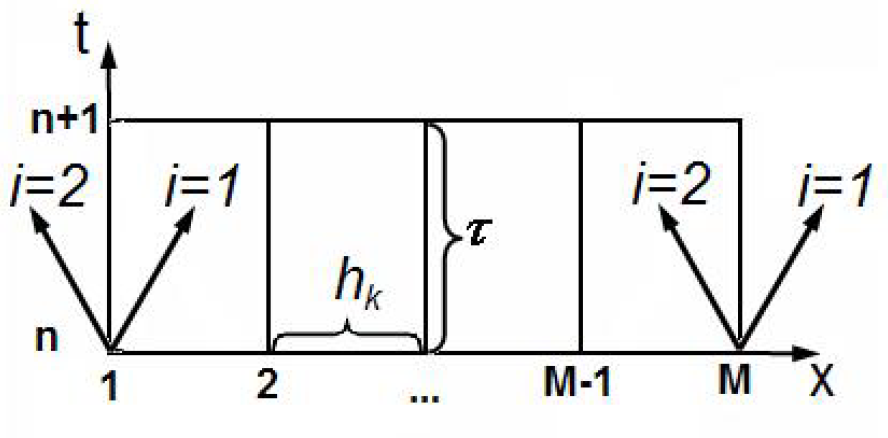
\includegraphics[scale=0.5]{char.png}
	\caption{Наклоны характеристик в узлах сеточного шаблона, соответствующим концам бронхиальной трубки} 
	\label{char}
\end{figure}

Дискретизация площади поперечного сечения на входе в носоглотку трахейно-бронхиального дерева может быть получена в результате подстановки уравнения \eqref{GrindEQ__3_} в уравнение \eqref{GrindEQ__6_}:
\begin{equation} \label{GrindEQ__35_} 
\left(S_{1} \right)_{0}^{n+1} =\left(1+\frac{p_{atm} }{\rho _{w} c_{01}^{2} } \right)S_{01}  
\end{equation} 
и использования уравнения \eqref{GrindEQ__33_} для расчета $\left(u_{1} \right)_{0}^{n+1} $.

Дискретизация граничных условий на выходе из трахейно-бронхиального дерева (точки стыковки терминальных трубок с альвеолярными компонентами) может быть получена следующим образом. С помощью неявной схемы Адамса второго порядка получим выражение \cite{GolovComp2017}:
\begin{equation} \label{GrindEQ__36_} 
V_{a}^{n+1} =V_{a}^{n} +0.5\tau\left(S_{J}^{n+1} u_{J}^{n+1}+S_{J}^{n} u_{J}^{n}\right) .  
\end{equation} 
Уравнения \eqref{GrindEQ__7_}, \eqref{GrindEQ__8_}, \eqref{GrindEQ__36_} используются для того, чтобы переписать уравнение \eqref{GrindEQ__9_} в форме:
\begin{equation} 
\label{GrindEQ__37_} 
\begin{array}
     \frac{128\eta }{9\pi ^{2} \left[V_{a}^{n} +0.5\tau\left(S_{J}^{n+1} u_{J}^{n+1}+S_{J}^{n} u_{J}^{n}\right) \right]} S_{J}^{n+1} u_{J}^{n+1} +\\+E_{a} \left[V_{a}^{n} +0.5\tau\left(S_{J}^{n+1} u_{J}^{n+1}+S_{J}^{n} u_{J}^{n}\right) -V_{0a} \right]=\rho c_{0}^{2} \left(\frac{S_{J}^{n+1} }{S_{0} } -1\right)-p_{pl}^{n+1} 
\end{array}
\end{equation} 

После подстановки уравнения \eqref{GrindEQ__31_} в уравнение \eqref{GrindEQ__35_} получается полиномиальное уравнение 4й степени относительно неизвестной переменной  $S_{J}^{n+1} $, которое решается с помощью метода Ньютона, при этом точка $S_{J}^{n} $ принимается за нулевое приближение метода. Численное исследование данного уравнения при физиологически адекватных значениях коэффициентов показало, что существует единственное корректное вещественное решение.  

Данный алгоритм хорошо сходится для используемых при расчетах шагов по времени, которые ограничены условием устойчивости численной схемы \eqref{GrindEQ__30_} и являются достаточно малыми относительно характерных времен дыхательных циклов $\left(\tau \approx 10^{-4} s\right)$.

\subsection{Численная реализация модели переноса дыхательных газов}
Расчет переноса дыхательных газов, описываемый уравнениям \eqref{GrindEQ__19_} -- \eqref{GrindEQ__26_}, выполняется после подсчета параметров потока, описанными выше алгоритмами. При этом значения площади поперечного сечения бронхиальных трубок, линейные скорости потока и объемы альвеолярных компонент на верхнем временном слое $\left(t=t_{n+1} \right)$ являются известными. 

Численный алгоритм разделяется на отдельный расчет внутренних узлов расчетной сетки бронхиальных трубок \eqref{GrindEQ__19_} с помощью схемы с разностью против потоков и граничных точек в областях бифуркаций бронхиальных трубок \eqref{GrindEQ__20_}, входе в носоглотку \eqref{GrindEQ__22_} и точках стыковки терминальных бронхиальных трубок и альвеолярных объемов \eqref{GrindEQ__22_}-\eqref{GrindEQ__26_}, которые в случае необходимости дополняются выражением неявной дискретизацией уравнения \eqref{GrindEQ__19_} полученной для необходимого терминального узла (вход или выход в бронхиальную трубку), если поток газа в этом узле направлен за пределы рассматриваемой бронхиальной трубки.

\subsection{Обработка данных компьютерной томографии}
Первоначальная 3D структура трахейно-бронхиального дерева была построена на основе анонимизированных CT-данных легких. Полученная информация использовалась как начальные данные для автоматической генерации 1D сетевой структуры в 3D пространстве и соответствующего графа бронхиальных трубок. Был применен алгоритм описанный в \cite{Danilov2016}. Данный алгоритм изначально успешно применялся для обработки индивидуальных данных структуры сосудов кровеносной системы. Алгоритм состоит из шага скелетонизации и шага построения структуры графа. Первая стадия алгоритма скелетонизации – это один из вариантов DOHT алгоритма \cite{Pudney1998}, на выходе которого которого получается начальный каркас для входных 3D CT-изображений. Искусственная структура в форме коротких сегментов также может быть получена на этой стадии. На второй стадии происходит удаление различного типа шумов (подробности описаны в \cite{Danilov2016}). На следующем этапе алгоритма элементы полученной скелетной структуры разбиваются на две группы: внутренние элементы и узловые элементы. Затем внутренние элементы конвертируются в ребра графа, а узловые элементы – в вершины графа. Также рассчитываются средние диаметры и длины сегментов графа. Готовая 1D сетевая структура легких была предоставлена автору. 

В расчетах использовалась сетевая структура вплоть до 4-го поколения ветвления, все остальные более мелкие структуры моделировались осредненно. Используемая в работе 3D сегментация и построенная на ее основе скелетная 1D структура показана на  Рис.~\ref{s2vechart}. Параметры сетевой модели отображены в Таб.~\ref{tab:langPuram}. Значения параметров $c_{0} $ были подобраны согласно литературным данным физиологии легких \cite{schmidt,Mead1961}.

\section{Программный комплекс}
\label{lung:soft}
Математическая модель и численные методы были реализованы в виде программного комплекса (Рис.~\ref{fig:soft_lung}). Программный комплекс состоит из трех основных компонент: модуля препроцессинга, решателя и модуля постпроцессинга. 
\begin{figure}[!ht]
	\centering
	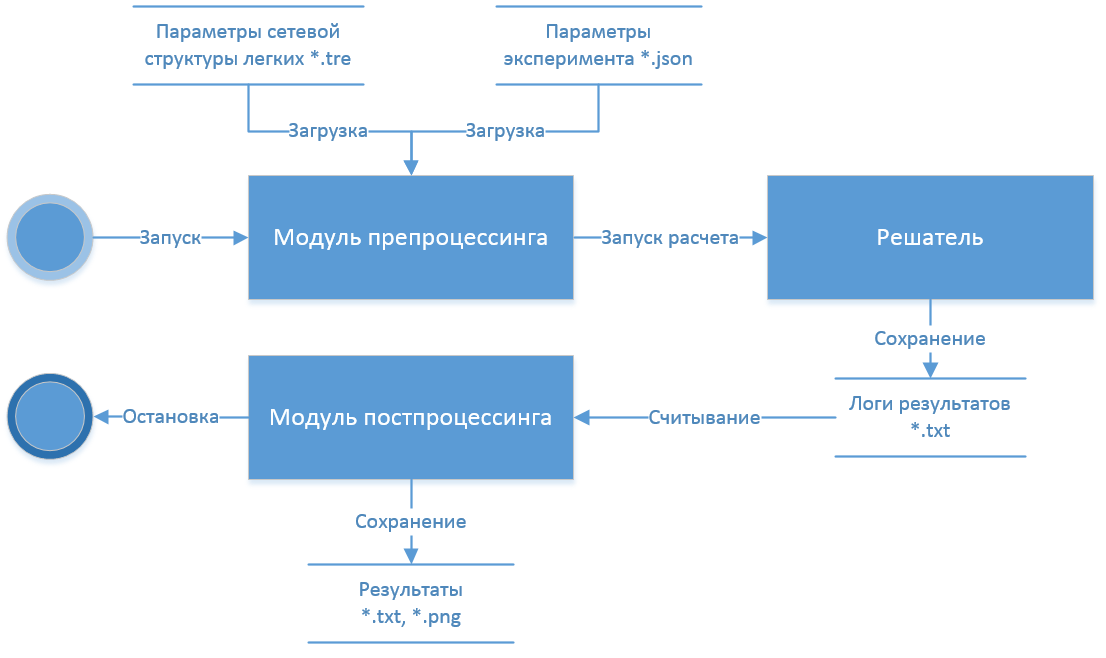
\includegraphics[scale=0.6]{pc4.png}
	\caption{Общая структура программного комплекса} \label{fig:soft_lung}
\end{figure}
В модуле препроцессинга происходит загрузка из конфигурационных файлов 1D сетевой структуры легких и параметров эксперимента (например моделирующих приступ астмы, патологические рисунки дыхания). На основе входных данных формируются параметры модели, которые поступают на вход решателя. Решатель производит расчет задачи и записывает логи эксперимента.
\begin{figure}[!ht]
	\centering
	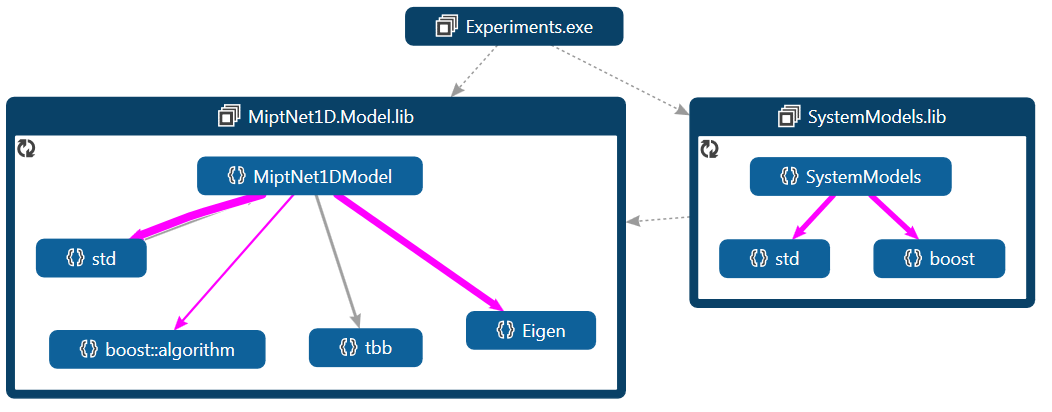
\includegraphics[scale=0.6]{pc1.png}
	\caption{Общая структура решателя} \label{fig:soft_solver}
\end{figure}
Данные модули написаны на языке C++ с использованием ООП парадигмы (Рис.~\ref{fig:soft_solver}). Выполнено разделение на две отдельные библиотеки.  В SystemModels.lib (Рис.~\ref{fig:soft_systems}) реализована абстрактная сущность организма человека, которая позволяет интегрировать  модели различных типов, масштабов, сложности и т.д., описывающих дыхательную, кровеносную, мышечную, нервную систем в единую глобальную модель. На основе данной абстрактной парадигмы реализовывалась, в том числе, и модель кровеносной системы и мышечного метаболизма из главы \ref{chapt:blood_muscle}.  
\begin{figure}[!ht]
	\centering
	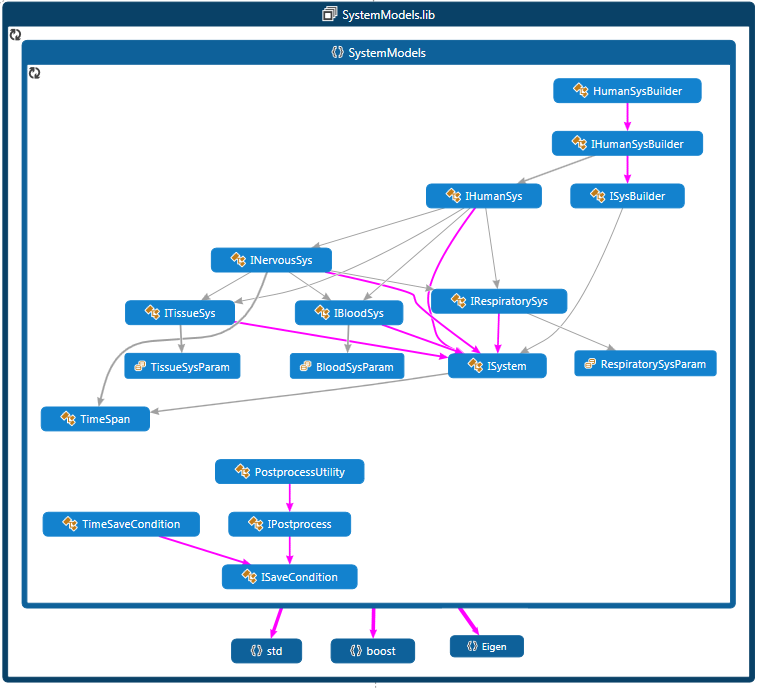
\includegraphics[scale=0.85]{pc3.png}
	\caption{Общая структура библиотеки SystemModels.lib} \label{fig:soft_systems}
\end{figure}

В MiptNet1D.Model.lib (Рис.~\ref{fig:soft_1d}) реализована совместная 0D-1D модель дыхательной системы, описанная в данной главе. В программной реализации использовались библиотеки Boost и Standard C++ Library. Для операций линейной алгебры использовалась библиотека Eigen. Для распараллеливания расчета в бронхиальных трубках, точках бифуркаций и альвеолярных объемах использовалась библиотека Intel Threading Building Blocks(TBB). Для расчета 60 сек. нормального синусоидального дыхания на двух ядерном Intel Core i3-2100 3.10GHz, Windows 7-64, 16Gb RAM требовалось в среднем 15 секунд.
\begin{figure}[!ht]
	\centering
	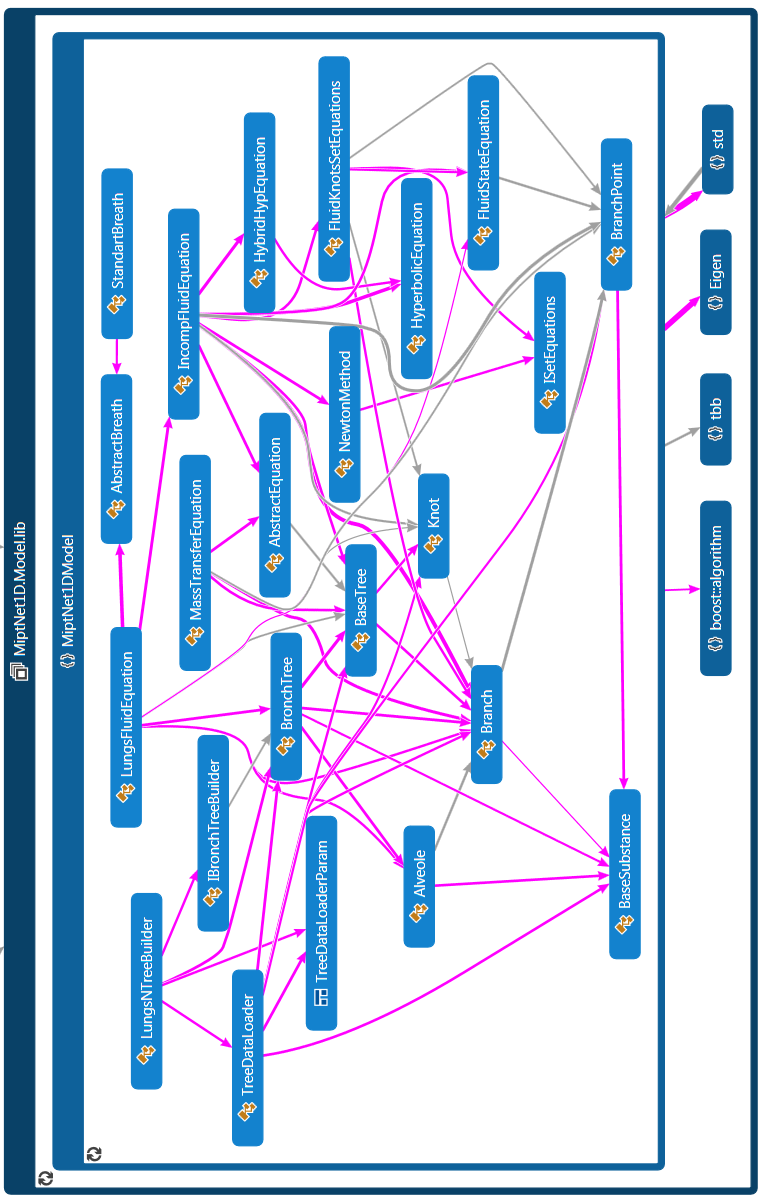
\includegraphics[scale=0.8]{pc2.png}
	\caption{Общая структура библиотеки MiptNet1D.Model.lib} \label{fig:soft_1d}
\end{figure}

После окончания работы решателя запускается модуль постпроцессинга, в котором считываются логи вычислительного эксперимента. На основе логов рассчитываются агрегированные характеристики, при необходимости выполняется визуализация. Данный модуль написан на языке Python с использованием библиотек Numpy, Pandas и Matplotlib.

\clearpage
\section{Резюме}
\begin{itemize}
\item
Для моделирования газообмена в легких, была выполнена декомпозиция их
структуры на проводящую зону (первые 4е поколения) и альвеолярные компоненты (8 компонент), каждая из которых осредняет альвеолы, альвеолярные ходы и бронхиолы.
\item
Движение воздуха в проводящей зоне легких  для каждой бронхиальной трубки описывается уравнениями сохранения массы и импульса, которые дополняются "уравнением состояния". Численный алгоритм позволяет разделить расчет на каждом шаге по времени на несколько этапов. На первом этапе с использованием явной двухшаговой гибридной схемы 1-2го порядка точности решаются уравнения во внутренних узлах расчетной сетки для каждой бронхиальной трубки. На втором этапе с помощью метода Ньютона решается система нелинейных алгебраических уравнений на входах, выходах, точках бифуркаций для каждой бронхиальной трубки в граничных узлах расчетной сетки, которая дополняется условием совместности вдоль соответствующих характеристик.
\item
Расчет переноса дыхательных газов ($O_{2}, CO_{2}$) выполняется после подсчета параметров потока. При этом значения площади поперечного сечения бронхиальных трубок, линейные скорости потока и объемы альвеолярных компонент на верхнем временном слое являются известными
\item
Перенос дыхательных газов ($O_{2}, CO_{2}$) в проводящей зоне описывается уравнением конвективного переноса. Численный расчет выполняется с помощью схемы с разностью против потоков. 
\item
Движение воздуха и перенос дыхательных газов в переходной зоне описывается интегральной моделью для каждого альвеолярного объема. Численный расчет уравнений модели выполняется совместно с уравнениями проводящей зоны для конечных бронхиальных трубок с использованием условий равенства давлений и сохранения массы. В итоге система сводится к нахождению корней полинома 4ой степени.  
\item 
1D сетевая структура легких, используемая при расчетах в проводящей зоне, получена на основе обработки CT-данных пациента (1D структура была предоставлена автору).
\item
Модель реализована в виде программного комплекса, состоящего из модулей препроцессинга, постпроцессинга и решателя. При реализации использовались языки программирования C++ и Python.  Для расчета 60 сек. нормального синусоидального дыхания на двух ядерном Intel Core i3-2100 3.10GHz, Windows 7-64, 16Gb RAM требовалось в среднем 15 секунд.
\end{itemize}